% This is samplepaper.tex, a sample chapter demonstrating the
% LLNCS macro package for Springer Computer Science proceedings;
% Version 2.20 of 2017/10/04
%
\documentclass[runningheads]{llncs}
\usepackage[T1]{fontenc}
\usepackage[utf8]{inputenc}
\usepackage{graphicx}
\usepackage{todonotes}

\begin{document}
%
\title{Classifier selection for imbalanced data streams with \emph{Minority Driven Ensemble}}
%
%\titlerunning{Abbreviated paper title}
% If the paper title is too long for the running head, you can set
% an abbreviated paper title here
%
\author{Paweł Zyblewski\orcidID{0000-0002-4224-6709} \and
Michał Woźniak\orcidID{0000-0003-0146-4205} \and
Paweł Ksieniewicz\orcidID{0000-0001-9578-8395}}
%
\authorrunning{P. Zyblewski et al.}
% First names are abbreviated in the running head.
% If there are more than two authors, 'et al.' is used.
%
\institute{Department of Systems and Computer Networks,\\ Faculty of Electronics, Wrocław University of Science and Technology,\\Wybrzeże Wyspiańskiego 27, 50-370 Wrocław, Poland
\email{\{pawel.zyblewski,michal.wozniak,pawel.ksieniewicz\}@pwr.edu.pl}}

\maketitle           

\begin{abstract}
The abstract should briefly summarize the contents of the paper in
15--250 words.
\keywords{First keyword  \and Second keyword \and Another keyword.}
\end{abstract}

%
\section{First Section}
\subsection{A Subsection Sample}
Please note that the first paragraph of a section or subsection is
not indented. The first paragraph that follows a table, figure,
equation etc. does not need an indent, either.

Subsequent paragraphs, however, are indented.

\subsubsection{Sample Heading (Third Level)} Only two levels of
headings should be numbered. Lower level headings remain unnumbered;
they are formatted as run-in headings.

\paragraph{Sample Heading (Fourth Level)}
The contribution should contain no more than four levels of
headings. Table~\ref{tab1} gives a summary of all heading levels.

\begin{table}
\caption{Table captions should be placed above the
tables.}\label{tab1}
\begin{tabular}{|l|l|l|}
\hline
Heading level &  Example & Font size and style\\
\hline
Title (centered) &  {\Large\bfseries Lecture Notes} & 14 point, bold\\
1st-level heading &  {\large\bfseries 1 Introduction} & 12 point, bold\\
2nd-level heading & {\bfseries 2.1 Printing Area} & 10 point, bold\\
3rd-level heading & {\bfseries Run-in Heading in Bold.} Text follows & 10 point, bold\\
4th-level heading & {\itshape Lowest Level Heading.} Text follows & 10 point, italic\\
\hline
\end{tabular}
\end{table}


\noindent Displayed equations are centered and set on a separate
line.
\begin{equation}
x + y = z
\end{equation}
Please try to avoid rasterized images for line-art diagrams and
schemas. Whenever possible, use vector graphics instead (see
Fig.~\ref{fig1}).

\begin{figure}
\includegraphics[width=\textwidth]{fig1.eps}
\caption{A figure caption is always placed below the illustration.
Please note that short captions are centered, while long ones are
justified by the macro package automatically.} \label{fig1}
\end{figure}

\begin{theorem}
This is a sample theorem. The run-in heading is set in bold, while
the following text appears in italics. Definitions, lemmas,
propositions, and corollaries are styled the same way.
\end{theorem}
%
% the environments 'definition', 'lemma', 'proposition', 'corollary',
% 'remark', and 'example' are defined in the LLNCS documentclass as well.
%
\begin{proof}
Proofs, examples, and remarks have the initial word in italics,
while the following text appears in normal font.
\end{proof}
For citations of references, we prefer the use of square brackets
and consecutive numbers. Citations using labels or the author/year
convention are also acceptable. The following bibliography provides
a sample reference list with entries for journal
articles~\cite{ref_article1}, an LNCS chapter~\cite{ref_lncs1}, a
book~\cite{ref_book1}, proceedings without editors~\cite{ref_proc1},
and a homepage~\cite{ref_url1}. Multiple citations are grouped
\cite{ref_article1,ref_lncs1,ref_book1},
\cite{ref_article1,ref_book1,ref_proc1,ref_url1}.


\section{Introduction}
Klasyfikacja taka ciężka. Niezbalansowana jeszcze cięższa. A przy strumieniach to już w ogóle.

To może selekcja klasyfikatorów \cite{cruz_deslib:2018}.

\section{Method}

\section{Set-up of experiments}

\subsection{Datasets}
\todo{Opis generatora}
\todo{Przegląd zbiorów syntetycznych}
\todo{Wypadałoby chyba jednak dodać te rzeczywiste, ale zróbmy to w następnym kroku}

\subsection{Experiments}

\subsubsection{Experiment 1 --- hyperparameters optimization}

Ustalamy typowy strumien zawierający problem o dużej skali niezbalansowania
(1:9) i szumie na poziomie udziału klasy mniejszościowej (.1). Testujemy
uśrednioną miarę i zależność statystyczną przebiegów dla różnych wielkości
komitetów i różnej wartości parametru odcięcia klasyfikatorów o przestarzałej
granicy decyzyjnej. Testujemy osobno strumień z dryfami nagłymi i
inkrementalnymi.

Oczekiwania:
- powiększanie komitetu początkowo stabilizuje jakość, ale z czasem degraduje
zdolność do reakcji na dryf koncepcji,
- zwiększanie progu odcięcia początkowo kompensuje spowolnienie reakcji na
dryf, ale z czasem wpływa negatywnie na stabilność jakości.
- obie wartości powinny być relatywnie niskie.
- czas trwania badań to około pół godziny.

\subsubsection{Experiment 2 --- comparative analysis of classifier selection methods}

\section{Experimental evaluation}

\subsubsection{Experiment 1 --- hyperparameters optimization}

Wyniki na Figure \ref{fig:experiment_1}.

\begin{figure}[hbt]
	\centering
	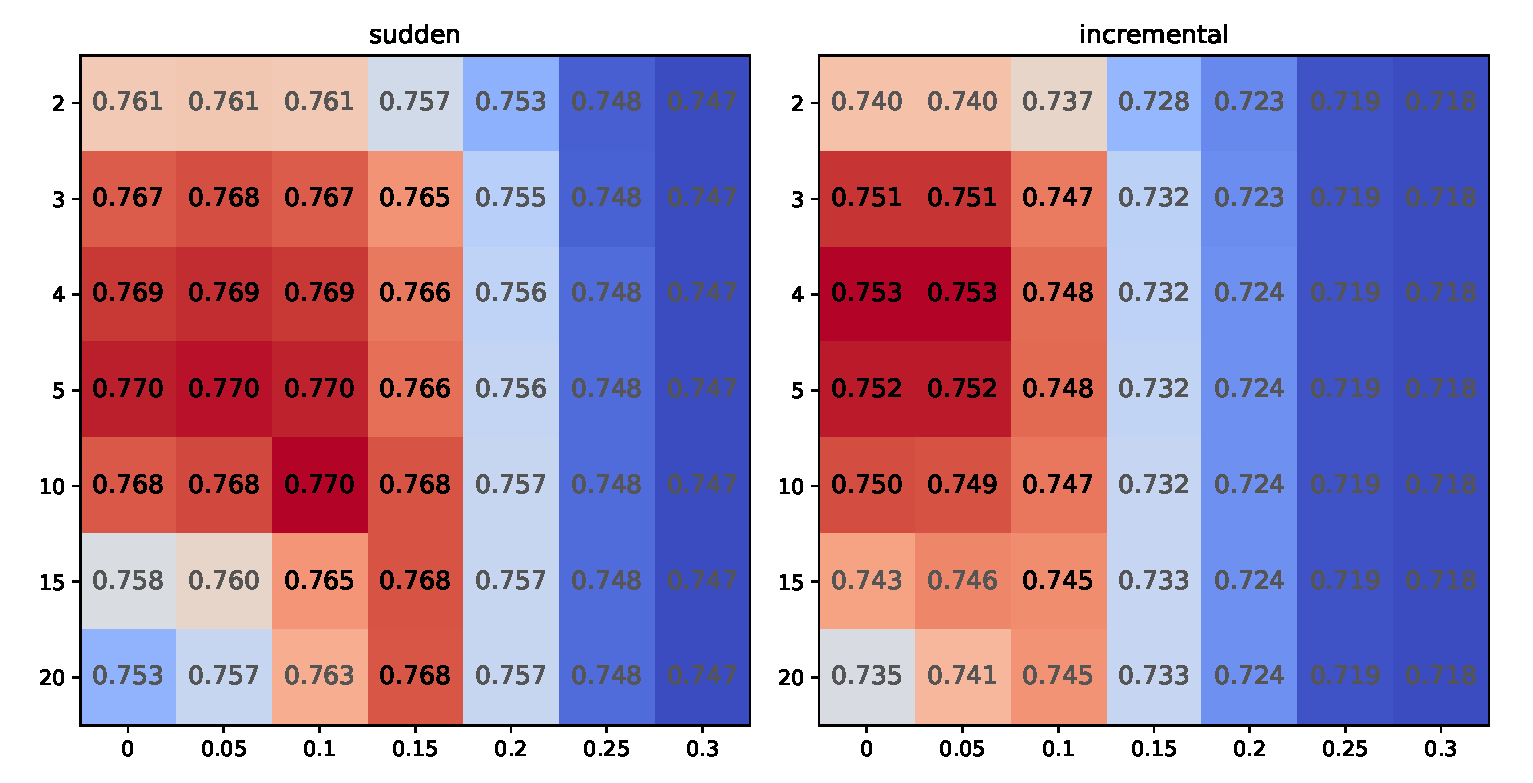
\includegraphics[width=.86\textwidth]{../figures/experiment_1}
	\caption{Podpis}
	\label{fig:experiment_1}
\end{figure}

Do dalszych badań wybrano komitet trzech klasyfikatorów i parametr alpha .05.

\subsubsection{Experiment 2 --- comparative analysis of classifier selection methods}

\section{Conclusions}

Jest super, akurat dla takich wspaniale nietypowych danych, które wcale nie są takie nietypowe.

\section*{Acknowledgement}

This work was supported by the statutory funds of the Department of Systems and Computer Networks, Faculty of Electronics, Wroclaw University of Science and Technology and by the Polish National Science Centre under the grant No. ???\todo{Numer grantu}.

%
% ---- Bibliography ----
%
\bibliographystyle{splncs04}
\bibliography{bibliography}

\end{document}
